%!TEX root = ../dokumentation.tex

\chapter{Praxis Kapitel}
\section{Einrichten der Entwicklungsumgebung}
Für den täglichen Gebrauch ist es nicht empfehlenswert Binaries als Root-User auszuführen. Um das HackRF One mit einem regulären Nutzer auf einem Linux System nutzen zu können, ist es notwendig eine entsprechende udev-Regel für das Gerät zu schreiben:

\begin{lstlisting}[caption=Erstellen einer udev-Regel, label=udev]
ATTR{idVendor}=="1d50", ATTR{idProduct}=="6089", SYMLINK+="hackrf-one-%k", MODE="660", GROUP="plugdev"
\end{lstlisting}

Die Datei mit der Regel wird unter /etc/udev/rules.d/ abgelegt. Verbindet man das Gerät nun mit dem Computer, wird ein Symlink unter /dev/ angelegt und Mitglieder der Gruppe \textit{plugdev} haben Zugriff darauf. 
Die erfolgreiche Installation kann durch das Ausführen des Kommandos \textbf{hackrf\_info} als User ohne root-Berechtigung überprüft werden:
\begin{lstlisting}[caption=Das Kommando "hackrf\_info" wird zum Test auf dem System ausgeführt, label=hackrfinfo]
hackrf_info version: git-a4c57ef
libhackrf version: git-a4c57ef (0.5)
Found HackRF
Index: 0
Serial number: 0000000000000000a06063c824237d5f
Board ID Number: 2 (HackRF One)
Firmware Version: 2017.02.1 (API:1.02)
Part ID Number: 0xa000cb3c 0x00544765
\end{lstlisting}


\newpage
\section{Grundbausteine in GNU Radio Companion}
GNU Radio Companion wird am besten durch das klassische FM-Radio Beispiel erklärt:

\begin{figure}[ht]
	\centering
	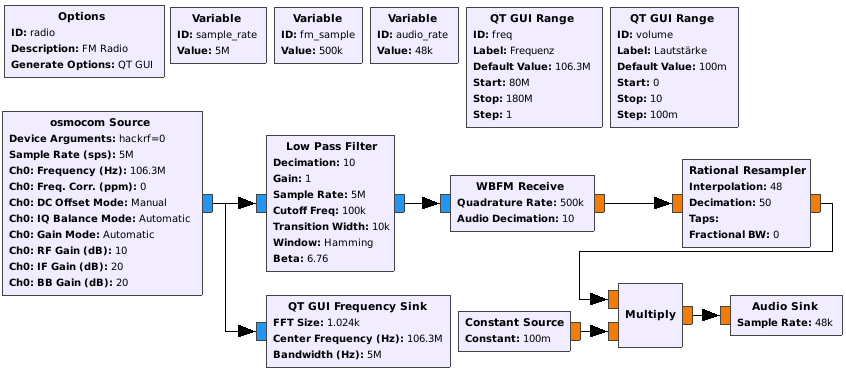
\includegraphics[width=\textwidth]{fmradio.png}
	\caption[Implementation eines FM-Radioempfängers in GNU Radio Companion]{Implementation eines FM-Radioempfängers in GNU Radio Companion. Quelle: Eigene Darstellung} 
	\label{fmradio}
\end{figure}

Das dargestellte Blockschaltbild realisiert das Empfangen, Demodulieren und Wiedergeben eines FM-Radio Signals. Das Programm bietet zudem die Möglichkeit Frequenz und Lautstärke anzupassen:

\begin{figure}[ht]
	\centering
	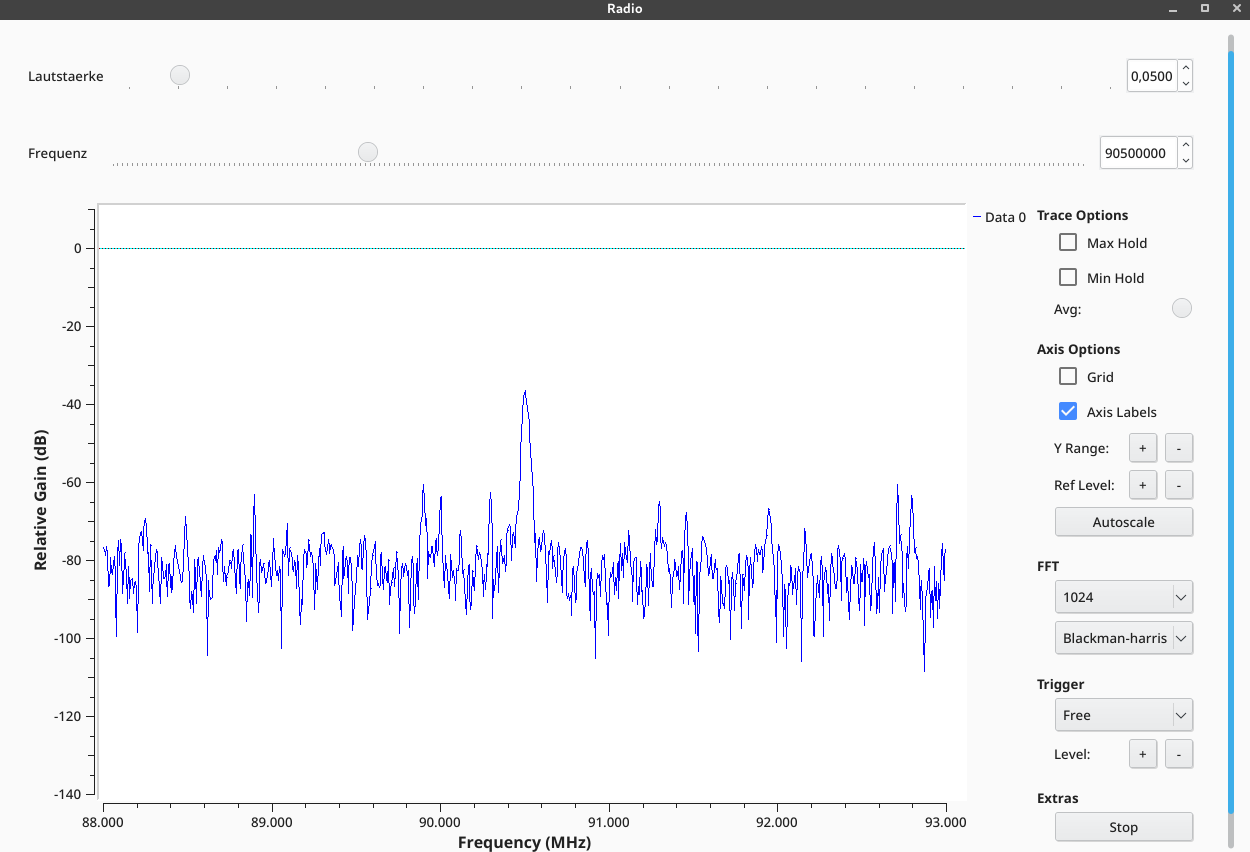
\includegraphics[width=0.8\textwidth]{fmradio-fft.png}
	\caption[FM Radio FFT-Plot]{FM Radio FFT-Plot. Quelle: Eigene Darstellung} 
	\label{fmradio-fft}
\end{figure}

Im Folgenden werden die einzelnen Bausteine näher erläutert.


\newpage
Als Signalquelle können in GNU Radio TCP/UDP Ports, Soundkarten, Dateien bzw. Input-Streams oder \ac{SDR}-Geräte benutzt werden.\newline
Um das HackRF One als Signalquelle zu verwenden, wird der quelloffene, von \ac{osmocom} \cite{osmocom:2018} entwickelte GNU Radio Block \textit{gr-osmosdr} \cite{gr-osmosdr:2018} benutzt.
Dieser untersützt das HackRF durch die zuvor installierte Bibliothek \textit{libhackrf}:

\begin{figure}[ht]
	\centering
	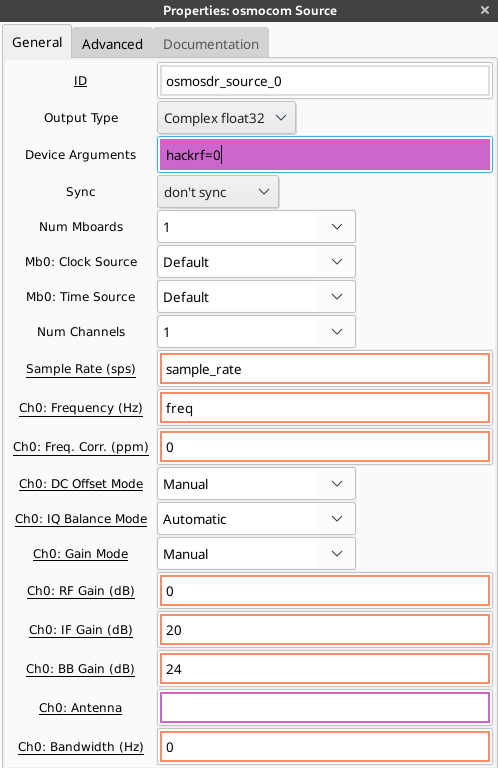
\includegraphics[width=0.5\textwidth]{osmocom-source.png}
	\caption[osmocom Source Block]{osmocom Source Block. Quelle: Eigene Darstellung} 
	\label{osmocom-source}
\end{figure}

\begin{description}
	\item[ID:] Der Name der Python-Variable des GRC Blocks
	\item[Output Type:] Der vom Block produzierte Datentyp, in diesem Fall \textit{Complex float32}, da das HackRF One Samples als IQ-Paare darstellt, wobei die I- und Q-Komponente jeweils als Float-Gleitkommazahl repräsentiert werden
	\item [Sample Rate (sps):] Die Abtastrate $f_a$ in Samples pro Sekunde
	\item[Ch0 Frequency (Hz):] Die Frequenz des Kanals. Da nur eine Antenne vorhanden ist, wird automatisch Channel 0 benutzt
	\item[Ch0 Freq. Corr. (ppm):] description %TODO
	\item[Ch0 RF Gain (dB):] description
	\item[Ch0 IF Gain (dB):] Intermediate Frequency
	\item[Ch0 BB Gain (dB):] Baseband
	\item[Ch0 Bandwidth (Hz):] Bandbreite
\end{description}
